\documentclass[acmtoms,acmnow]{acmtrans2m}
%&t&{\tt #}&
%&v&\verb|#|&

% fancybox prevents the TOC from printing
%\usepackage{fancyhdr, fancybox, tabularx, verbatim, epsfig}
\usepackage{fancyhdr, tabularx, verbatim, epsfig}
\usepackage{amssymb,psboxit}
\usepackage{rotating}
\usepackage{tabularx}

\newcommand{\amesos}{{\sc Amesos}}

\acmVolume{0}
\acmNumber{0}
\acmYear{00}
\acmMonth{00}

\newtheorem{interface}{Interface}[section]
\newtheorem{remark}{Remark}

\newcommand{\BibTeX}{{\rm B\kern-.05em{\sc i\kern-.025em b}\kern-.08em
    T\kern-.1667em\lower.7ex\hbox{E}\kern-.125emX}}

\markboth{M. Sala, K. Stanley and M. Heroux}{Interfaces to Sparse Direct Solvers}

\title{On the Design of Interfaces to Sparse Direct Solvers}

\author{MARZIO SALA \\
Eidgen\"ossische Technische Hochschule Z\"urich \\
KENDALL S. STANLEY \\
Oberlin College \\
 and MICHAEL A. HEROUX \\
 Sandia National Laboratories}

\begin{abstract}
We discuss the design of general, flexible, consistent, reusable and
efficient interfaces to software libraries for the direct solution
of systems of linear equations on both serial and distributed memory
architectures. We introduce a set of abstract classes to access the
linear system matrix elements and their distribution, access vector
elements, and control the solution of the linear system.

We describe a concrete implementation of the proposed interfaces,
and report examples of applications and numerical results showing
that the overhead induced by the object-oriented design is
negligible under typical conditions of usage. We include examples of
applications, and we comment on the advantages and limitations of
the design.
\end{abstract}

\category{D.1.3}{Programming Techniques}{Parallel Programming}
\category{D.2.2}{Software Engineering}{Design Tools and Techniques--{\sl
 Object-oriented design methods}}
\category{D.2.13}{Software Engineering}{Reusable Software--{\sl Reusable
  libraries}}
\category{G.1.3}{Numerical Analysis}{Numerical Linear Algebra--{\sl
  Sparse, structured, and very large systems (direct and iterative methods)}}
%\terms{Documentation, Languages}

\keywords{Direct Solver Libraries, Object-Oriented Design, Distributed Linear Algebra.}
\begin{document}


\setcounter{page}{1}

\begin{bottomstuff}
Authors' address:
\newline Marzio Sala: Department of Computer Science, ETH Z\"urich, CH-8092 Z\"urich,
  Switzerland.
\newline Ken Stanley: Department of Computer Science, Oberlin College, Oberlin, Ohio,
  USA.
\newline Michael A. Heroux: PO Box 5800 MS 1320, Albuquerque, NM 87185-1320,
U.S.A.
\newline ASC program and the DOE Office of Science MICS
program at Sandia National Laboratory.  Sandia is a multiprogram
laboratory operated by Sandia Corporation, a Lockheed Martin
Company, for the United States Department of Energy's National
Nuclear Security Administration under contract DE-AC04-94AL85000.
\end{bottomstuff}

\maketitle

% --------------------------------------------------------------------------- %
\section{Motivations}
\label{sec:introduction}
% --------------------------------------------------------------------------- %

This paper describes the design and the implementation of
interfaces to libraries for the serial and parallel direct solution of
linear systems of type
\begin{equation}
  \label{eq:linear_system}
  A x = b,
\end{equation}
where $A \in \mathbb{R}^{n \times n}$ is a real and sparse square matrix,
  and $x, b \in \mathbb{R}^{n}$ are the solution and
the right-hand side vectors, respectively.

Generally speaking,
a direct solution algorithm for (\ref{eq:linear_system}) is any
technique that computes three matrices, $L$, $D$ and $U$, such that
$P\, A\, Q = L \, D \, U$, where $P$ and $Q$ are permutation matrices
and the linear systems with matrices $L$, $D$ and $U$ are
easy to solve~\cite{golub96matrix}.
The process of computing these three matrices is called {\sl
  factorization}. Typically, $L$ is a lower triangular matrix, $U$ is an
upper triangular matrix, $D$ is a diagonal matrix
(or possibly the identity matrix), and the algorithm adopted for their
computation is some variant of the Gaussian elimination method.

Direct sparse solvers are an essential kernel in scientific and
engineering computing and are required by several numerical
algorithms, even within the same application. An incomplete list
would include implicit time-stepping schemes, Newton-like methods,
multilevel and domain decomposition preconditioners. In some
instances these solvers are applied to the original problem in
(\ref{eq:linear_system}). Increasingly these solvers are used as a
phase of a more complex solution process where the direct solver is
used as a coarse grid problem solver, or is used to solve a set of
subproblems, such as in FETI~\cite{FETI} methods.  Thus, even though
the parallel scalability of direct sparse solvers is usually limited
to a factor of 10-100 speedup, these solvers remain a critical
technology for large-scale simulations.

The development and implementation of
direct solvers for (\ref{eq:linear_system}) is a
challenging task that has been a subject of research over the
last four decades.
A brief overview of direct solution algorithms  is given in
Section~\ref{sec:overview}; however,
the focus of this article is on the {\sl usage} of direct solution methods,
    rather than on their development or analysis.
Therefore, the point of view is the one of users (that is, application
                                                  developers),
that are interested in solving
(\ref{eq:linear_system}) using already available software libraries.

\smallskip


In contrast with dense solvers, where one can take advantage of the
widely-available suite of solvers contained in the LAPACK
library~\cite{lapack-guide} and ScaLAPACK
library~\cite{scalapack-guide} or the PLAPACK
library~\cite{alpatov97plapack}, there is no single direct solver
library of choice for (distributed) sparse linear systems. Since no
``gold standard'' exists, application developers aiming to solve
(\ref{eq:linear_system}) generally have to look for a suitable
library that meets their needs. This search is affected by the
following questions:
\begin{enumerate}
\item[(Q1)] Software ease-of-use and availability: Is the software library easy to use,
stable, well-documented and actively supported?  
Is it portable to all required platforms and 
does it have an acceptable licensing agreement?
\item[(Q2)] Special numerical properties:  Does the solver support the special properties of my problems?
For example, does the solver support symmetric matrices, reuse of
matrix patterns, robust pivoting, etc.?
\item[(Q3)] Time-to-solution: Is the solver efficient in terms of CPU time?
\item[(Q4)] Memory use: How much storage does the solver require?
\end{enumerate}
The relative importance of these aspects is usually subjective. For small
problems Q1 and Q2 are critical, since both time-to-solution and memory use
will be irrelevant.
For possibly large but relatively well-conditioned problems, (Q3) is usually the key point, followed
by (Q4). For complicated problems, and especially in industrial
applications, (Q2) is of paramount importance. (Q1) is often
considered part of the ``technical details'' of minor importance,
even if they are truly important.  At this time there are many viable
direct sparse solvers, each of which has a special ``niche'' in the
user community because it addresses the above questions
appropriately for some users.

Using libraries can be a non-trivial task, since library developers
often include a wide variety of choices, aiming to provide a
powerful and comprehensive library. Furthermore, many solver
parameters are \textit{ad hoc} and users have little \textit{a
priori} sense of optimal parameter values.  Application developers,
in contrast, are usually not experts in direct sparse solvers, and
do not aim to become such. They often choose the code that looks
easier to use and seems to perform in a reasonable way. This
difference of views creates a gap between the actual and potential
use of mathematical software. Of course, a simple but inefficient
library is of no interest; therefore the ``optimal'' library will
exhibit a mixture of the features outlined above.

Once a library has been chosen, the application developers have to
write a custom-made interface between the selected library and
the application. This usually requires storing the linear system matrix $A$
using the
  storage format required by the library, then calling the correct sequence of
  instructions to factor the matrix and solve the linear system.  In our
  opinion, the above approach is sub-optimal for both application and library
  developers because it:
\begin{enumerate}

\item
{\sl Offers partial coverage:} Writing a custom-made interface means
that only the targeted library will be used. This is inconvenient
because of the already mentioned difficulty to {\it a-priori} choose
the best library for a given application. In some cases, a
theoretical analysis of the problem at hand can suggest the right
algorithm. Alternatively, one can consider numerical comparisons on
test matrices available in the literature, see for instance
\cite{amestoy01analysis,gupta01recent,golub05numerical} and the
references therein. Often, however, one has to validate a given
library on the application, architecture, and data set of interest,
and this can be done only if the interface is already available;

\item
{\sl Produces maintenance problems:} Including the interfaces within
the application code requires the application developers to
manipulate the matrix format, the memory management, the calling
conventions, and others, that can vary from one library to the
following. Although not necessary difficult, these activities are
usually time-consuming;

\item
{\sl Delays the usage of new libraries:} Large application codes
usually have a long life.  The sheer size of the codes and a natural
reluctance to change successful projects discourage any effort of
rewriting unless absolutely necessary. Since a new library (or a new
version of a given library) may require a new matrix format or
distribution, or new calling conventions, application developers may
simply decide to continue using the interface already developed.
\end{enumerate}

This article shows that it is possible to address these problems by
using object-oriented (OO) design and programming.  We propose a set
of clean, consistent and easy-to-use interfaces between the
application and the direct solver libraries.  Each interface takes
care of dealing with the direct solver library, in a manner that is
transparent to the application developers, and automatically manages
matrix formats, data layout, and calling conventions. Our design is
based on the following requirements:
\begin{enumerate}

\item {\sl Simplicity of usage:} Solving linear system
(\ref{eq:linear_system}) in a language like MATLAB is very easy, i.e.~one just
writes \verb!x = A \ b!. It should not be much different in a non-MATLAB
code;

\item {\sl Flexibility:} More than one algorithm/library must be available,
  for both serial and parallel architectures;

\item {\sl Efficiency:} The overhead due to the framework must be minimal.
\end{enumerate}

The basic ideas of our design are indeed quite old, and can be traced back to
almost 30 years ago~\cite{duff79performance,george79design}. More recently,
  articles~\cite{george99object,dobrian99design} discussed the usage of
  abstract interfaces and OO design for the direct solution of sparse linear
  systems.  We extend these ideas by abstracting the concepts to
a higher level, and making the interfaces independent of the
supported libraries. The interfaces are presented and implemented as
a set of C++ classes using several well-known design
patterns~\cite{Gamma}. C++~\cite{cppbook} supports object-oriented
programming, and it is relatively easy to interface FORTRAN77,
FORTRAN95 and C libraries with C++ code. C++ supports abstraction
through classes, inheritance and polymorphism. For application
developers, abstraction is important because it enhances simplicity,
by providing components with a minimal interface. It also ensures
flexibility because it decouples the different algorithmic phases
from the data structures. Finally, abstraction allows extensibility
in the sense that new (yet to be developed) libraries can be easily
added, at almost no cost to the application developer. Another
candidate language could have been FORTRAN95, but it does not have
inheritance and polymorphism.

%
%  I think that we can be more direct about our dependence on MPI here.
%
Regarding the parallel computing mode, we consider parallel
architectures with distributed memory, and we assume that the
message passing interface MPI~\cite{gropp98mpi} is adopted. This
approach is followed by several scientific libraries, see
\cite{heroux05trilinos,petsc-user-ref,falgout02hypre}. As a result,
the presented design can be easily interfaced with the
aforementioned projects.

\smallskip

The paper is organized as follows. Section~\ref{sec:overview} introduces the
basic concepts of direct solution algorithms. Section~\ref{sec:design}
describes the requirements and the design of the proposed
interfaces. A concrete implementation is addressed in
Section~\ref{sec:concrete}. Section~\ref{sec:numerical} reports some
numerical results that quantify the overhead required by the generality of
the approach. Two
examples of application are reported in Section~\ref{sec:example}.
Section~\ref{sec:conclusions} outlines the conclusions.

%-----------------------------------------------------------------------------
\section{Brief Overview of Direct Solution Methods}
\label{sec:overview}
%-----------------------------------------------------------------------------

This section gives a broad view of the challenges of Gaussian
elimination algorithms for distributed sparse linear systems. For
more details on the subject, the interested reader should consult
the specialized literature, for
example~\cite{duff86direct,duff97sparse} and the references therein.

Following~\cite[Chapter 6]{dongarra98numerical}, a direct solution algorithm
for sparse matrices can be divided in the following phases:
\begin{itemize}
\item[(S0)] Preordering:  This phase
determines a reordering of the original matrix such that fill is
reduced in the $L$ and $U$ factors.  This phase is difficult to
parallelize and is typically computed redundantly on a parallel
machine, or on a single processor with results then broadcast to
other processors.
\item[(S1)] Analysis:  Here the factorization is computed
using the structure only, producing the patterns of $L$ and $U$.  In
particular, many solvers use this phase to identify dense supernodes
that will improve cache and register performance; and also determine
elimination trees for additional parallelism during the numerical
phases (S2) and (S3).
\item[(S2)] Numerical factorization: In this phase, the actual values
of $L$ and $U$ are computed.  In most cases this phase is by far the
most expensive in terms of serial operation count. However, this
phase also tends to have the best single processor and parallel
machine utilization of any phase.  Thus, on high-performance
computers, the wall-clock time of this phase will improve greatly,
relative to other phases.  However, it is rare to see more that a
factor of 50 times speedup, even on hundreds of processors.
\item[(S3)] Forward/Back solve:  This phase finds a solution $x$ given $b$.
Compared to the factorization, the serial cost of this phase
is low, perhaps by a factor of 10--100 or more.  However, this phase
tends to have poor parallel scaling and does not perform as well as
the factorization phases on modern processors.  Therefore, the cost
of repeated forward/back solves (using the same factors $L$ and $U$)
on a parallel machine may actually become the most expensive phase.
\end{itemize}
Some codes combine phases (S1) and (S2). Phase (S0) is typical of
sparse matrices: since $A$ is sparse, $L$ and $U$ are still sparse,
though they may have some fill-in, i.e. non-zero entries which are
zero in $A$. Therefore, the factorization is performed on $PAQ$. In
a typical solver for an unsymmetric matrix, the column permutation,
$Q$ is chosen to minimize fill-in, while $P$, the row permutation,
is chosen to maintain numerical stability.
%Pivoting for numerical
%stability makes it impossible to know in advance how the algorithm
%will proceed and requires a flexible data structure.  This is
%particularly difficult for distributed memory codes.
Many ordering methods exist to reduce fill-in, for example multiple variations
on minimum degree orderings and graph partitioning algorithms.  Solvers
designed for symmetric and nearly symmetric matrices typically use symmetric
permutations to maintain symmetry.  No single ordering method is best for all
matrices, nor has a heuristic been found that consistently chooses the best
ordering~\cite{BaumannFleischmannMutzbauer03,AmestoyDavisDuff03}.

Since pivoting adds complexity, which significantly increases
execution time, many solvers offer options to reduce the cost of
pivoting~\cite{LiDemmel509092,sg:04-fgcs}.  Some equilibrate the
rows and columns of the matrix to improve diagonal dominance.  Many
codes will consider the effect on execution time when choosing a
pivot, accepting some loss of numerical
stability~\cite{Malard126136}. Typically this just means accepting
the diagonal pivot if it is within some threshold of the best
available, but some codes will take the predicted effect on
execution time into consideration when choosing an off diagonal
pivot~\cite{Davis992205}.

It is possible to combine similar rows and columns into blocks to
improve locality and allow high performance BLAS to be called; this
combination can consider only rows and columns that are identical,
or accept minor differences in the rows and columns that they treat
as blocks.  Such blocking can reduce the cost of symbolic
factorization as well~\cite{amestoy01analysis}.

We have just mentioned a few reasons that explained why
the performance of a sparse direct solver depends on the underlying
matrix, computer, application, algorithms, and libraries as well as
the code and how it is compiled.
Given the differences in matrix, computer, application, algorithms,
and libraries, it is unlikely that a single sparse direct solver will
outperform all others across all usages.



%Although a solver designed for an
%unsymmetric matrix will work on symmetric matrices, solvers designed
%for symmetric matrices will typically be faster on symmetric matrices.
%Codes designed for shared memory computers will not run on distributed
%memory computers.  Codes designed for distributed memory computers can
%work on shared memory computers, but cannot take full advantage of the
%shared memory architecture.  Many applications require repeated solves
%with little or no difference in the matrix between solves.  Some
%algorithms are able to take advantage of the similarity in matrices
%between solves.

%The different characteristics of the matrices which users wish to
%solve impact sparse direct solvers.  Some matrices are symmetric in both
%structure and data $A_{i,j} = A_{j,i}$ for all $i$ and $j$.  Some of
%the symmetric matrices are positive definite, SPD, and require no
%pivoting.  The most efficient algorithms for symmetric and SPD
%matrices will not work on other matrices.  Some matrices are symmetric in
%structure, $A_{i,j} == 0$ iff $A_{j,i} == 0$, or nearly so.
%Algorithms that maintain symmetry typically outperform others on
%matrices with symmetric or nearly symmetric structure.  Some matrices have many
%columns and/or rows that are structurally identical, or nearly so.
%Aggregating nearly identical rows and columns into blocks allows more
%efficient BLAS3 routines to be used.  Some matrices can be factored with little
%fill-in, others require significant fill-in.  Matrices that can be
%factored with little fill-in and have few identical or nearly identical
%rows and columns are best handled by a low overhead code that does not
%use the BLAS.  Some matrices are banded or nearly so, allowing the use
%of a banded solver.  Matrices that have a non-trivial reduction to
%block triangular form can be solved more quickly, often dramatically,
%by a solver that includes reduction to block triangular form.  No sparse direct solver is best for all types of matrices.
%
%% MS % This seems to generic to me... Maybe re-write?
%Some sparse direct solvers are designed for single processor
%computers, some are designed for shared memory computers and others
%are designed for distributed memory computers.  Solvers designed for
%single processor computers can, if they use the BLAS for much of their
%computation, achieve some speedup on shared memory computers.
%Likewise, solvers designed for distributed memory computers can work
%on shared memory computers using an MPI interface.  However, only
%codes designed for shared memory computers can take advantage of the
%shared memory architecture.  Codes designed for shared memory
%computers will not work on distributed memory computers.  No single
%code will provide optimal performance across all architectures.

%Some solvers handle certain application requirements better than
%others.  Most applications perform a series of solves, possibly
%involving similar or even identical matrices.  If the matrix does not
%change between two consecutive solves, the symbolic and numeric
%factorization phases need not be performed for each solve.  If the
%structure of the matrix does not change between consecutive solves,
%but the values do, the numeric factorization must be performed for
%each solve, though the symbolic factorization phase need not be.  If
%the matrix values change, but the change is modest, the pivot order
%may not need to change.  Therefore, some applications care most about
%the execution time of the solve phase, while others are most sensitive
%to the execution time of the factorization (numeric and/or symbolic).
%Some applications require more accuracy than others.

%The three common methods for exploiting parallelism are the
%multi-frontal method, coalescing  similar
%columns into blocks and calling a parallel dense solver
%to factor the final block of the matrix~\cite{amestoy01analysis}.

% MS % discussed in the conclusions: skip it here?
%
% Some solvers allow incomplete factorizations which ignore small
% elements in the original matrix and/or the $L$ and $U$ factors.
% This feature is used primarily by users seeking a
% preconditioner for an iterative method.

%Some solvers use iterative refinement to improve accuracy.  Iterative
%refinement is used most often with codes that do not perform full partial pivoting.

%-----------------------------------------------------------------------------
\section{Project Design}
\label{sec:design}
%-----------------------------------------------------------------------------

%\begin{table}
%\begin{center}
%\begin{tabular}{| l | c c c l l | p{4cm} |}
%\hline
%package &
%\rotatebox{90}{complex} &
%\rotatebox{90}{parallel} &
%\rotatebox{90}{out-of-core} &
%\rotatebox{90}{language} &
%method &
%references \\
%\hline
%%
%CHOLMOD     & $\bullet$ & -- & -- & C & left-looking supernodal &
%\cite{davis05cholmod} \\
%%
%DCSPACK     & $\bullet$ & -- & D & C & multifrontal & \cite{dscpack-manual} \\
%%
%KLU         & $\bullet$ & -- & -- & C & left-looking & \cite{davis05klu} \\
%%
%Mathematica & $\bullet$ & -- & -- & -- & various & \cite{wolfram99mathematica} \\
%%
%MATLAB      & $\bullet$ & -- & -- & -- & various & \cite{gilbert92sparse} \\
%%
%MUMPS       & $\bullet$ & D & -- & F90 & multifrontal & \cite{mumps-manual} \\
%%
%Oblio       & $\bullet$ & -- & $\bullet$ & C++ & left, right, multifrontal &
%\cite{dobrian00oblio} \\
%%
%PARDISO     & $\bullet$ & S & -- & C & left/right supernodal  & \cite{oskl:04-etna,sg:04-fgcs} \\
%%
%%%PaStiX      & $\bullet$ & D &  ?? & -- & left-looking supernodal & \cite{henon00pastix} \\
%%
%TAUCS       & $\bullet$ & S & $\bullet$ & C & left-looking, multifrontal &
%\cite{irony04parallel,rotkin04design,rozin04locality} \\
%%
%UMFPACK     & $\bullet$ & -- & -- & C & multifrontal & \cite{umfpack-home-page} \\
%%
%SPOOLES     & $\bullet$ & S/D & -- & C & left-looking, multifrontal & \cite{ashcraft99spooles} \\
%%
%SuperLU     & $\bullet$ & -- & -- & C & left-looking supernodal &  \cite{superlu-manual} \\
%%
%SuperLU\_DIST & $\bullet$ & S & -- & C & left-looking supernodal &  \cite{superlu-manual} \\
%SuperLU\_DIST & $\bullet$ & D & -- & C & right-looking supernodal & \cite{superlu-manual} \\
%WSMP & $\bullet$ & S/D & -- & binaries & multifrontal & \cite{gupta02improved} \\
%%%Y12M & -- & -- & -- & F77 & right-looking Markowitz & \cite{y12m} \\
%
%
%\hline
%\end{tabular}
%\caption{Package features. `--' means that the feature is not supported. `S'
%  indicates support for shared memory machines, `D' for distributed memory
%    machines.}
%\label{tab:packages}
%\end{center}
%\end{table}

An analysis of currently available direct solver libraries can be found
in \cite{davis05summary}; see also~\cite[Section 6.7]{dongarra98numerical}.
A closer look at these solvers reveals the following major
differences:
\begin{enumerate}
\item {\sl Different programming languages are used:} This is true even if most projects are
written in C.

\item {\sl Different communication paradigms are used:}
 Most of the reviewed libraries are serial, some are based on the MPI
 paradigm, others take advantage of shared memory parallel computers.

\item {\sl Different matrix formats and data layouts are used:}
Most of these differences are small.

\item {\sl Different algorithms are used:} The underlying algorithms differ
and can therefore perform differently, depending on the considered matrices and
computer architectures.

\end{enumerate}

Despite the above differences between specific solvers, all solvers
are accessed within a given application by using a sequence of steps
similar to steps (S0)--(S3) of Section~\ref{sec:overview}.  Here we
show these application steps (A1)--(A3) in relation to (S0)--(S1):
\begin{enumerate}
\item[(A1)] Definition of the sparsity pattern of the linear system matrix;
\item[(S0/S1)] Computation of the symbolic factorization, which includes
preordering and analysis. The
symbolic factorization refers to all operations that can be performed by
accessing the matrix structure only (without touching the values of the matrix entries);
\item[(A2)] Definition of the values of the linear system matrix;
\item[(S2)] Computation of the numeric factorization, that is, the computation
of the entries of the factored terms;
\item[(A3)] Definition of the right-hand side $b$;
\item[(S3)] Solution of the linear system, that is, computation of $x$.
\end{enumerate}
Steps (A1)--(A3) are application-dependent and will not be discussed
here; instead, our aim is to standardize steps (S0/1), (S2) and (S3)
by adding an intermediate layer between the application and the
direct solver libraries.

The design discussed below uses several common \textit{design
patterns}~\cite{Gamma}.  Design patterns are commonly occurring
approaches to organizing software and are language independent,
although their popularity has grown with the increasing use of
object-oriented languages. In fact they are so common that
programming experts recognized frequent patterns and eventually
developed a common classification of patterns, standardizing
terminology and reducing incidental variations on the patterns, all
with the purpose of promoting rapid development of understandable,
reusable software.

In our work, we have adopted several common design patterns and
briefly mention them for the interested reader. In addition to the
classic Gamma reference~\cite{Gamma}, a very readable presentation
of design patterns can be found in~\cite{HeadFirstDesignPatterns}.
The first pattern we discuss is the \textit{Builder Pattern}, by
which we define an abstract class whose methods are steps
(S0)--(S3). Because each of these steps could in principle be
replaced with an alternate algorithm, our design also represents the
\textit{Strategy Pattern}, which exactly defines this situation.
Finally, we use the \textit{Factory Pattern} as a means of selecting
a specific concrete solver instance by use of a string argument.  A
factory can be used to produce an instance of a particular concrete
class that is also adapted to behave like a common generic base
class. In our context the factory can produce a specific solver
instance for any of the supported solvers, e.g., UMFPACK, SuperLU,
etc.  In addition, the factory passes the solver instance back as a
generic \amesos\ solver. In this way, regardless of which specific
solver was created, it is treated as a generic \amesos\ solver.

Presently we introduce a set of abstract classes that will be used
to define interfaces to the data layout of distributed objects,
vectors, matrices, linear system, and the solver. The design is
reported here as a set of C++ classes, but the concepts are more
general and the discussion, much like design patterns, is largely
language-independent. We only consider {\tt int} and {\tt double}
data types because our concrete implementation of the presented
design, described in Section~\ref{sec:concrete}, currently does not
support templates. However, one could easily exploit the C++ support
for genericity, and replace {\tt int} and {\tt double} with
templated data types, for example \verb!float! or
\verb!complex<double>!.

\smallskip

The first class that we need to introduce is a {\tt Map}, which defines the
data layout of the elements contained in vectors and matrices\footnote{This
class should not be confused with the STL {\tt map} class.} {\tt Map}'s
are also used to specify the local-to-global numbering, and the global and
local number of elements.  The {\tt Map} class is defined by
\begin{interface}
\label{int:map}
The {\tt Map} class will contain the following methods:

\begin{itemize}
\item {\tt int getNumMyElements() const} returns the number of locally owned elements;
\item {\tt int getNumGlobalElements() const} returns the global number of elements;
\item {\tt int getGID(const int LID) const} returns the global ID of the local node {\tt ID}.
\end{itemize}
\end{interface}

Note that it is trivial to implement the {\tt Map} class when working on
serial architectures. For parallel architectures, the {\tt Map} class
only requires that any global ID is assigned to exactly one processor.

The next class is the {\tt Vector}
class, which specifies the interfaces for
distributed vectors\footnote{
For the sake of simplicity, this paper focuses on vectors and not on
multi-vectors, that is, a collection of vectors with the same {\tt Map}.
However, the presented design can be straightforwardly extended to tackle
multi-vectors as well.
}. We assume that {\tt Vector}'s  locally exist as a {\tt double} arrays.
A simple set of methods for the {\tt Vector} class is reported by
\begin{interface}
\label{int:vector}
The {\tt Vector} class will contain the following methods:

\begin{itemize}
\item {\tt double* getValues()} returns a pointer to the local array of values;
\item {\tt const double* getValues() const} returns a pointer to the local
array of values for constant objects;
\item {\tt const Map\& getMap() const} returns a reference to the underlying Map object.
\end{itemize}
\end{interface}

Methods {\tt getValues()} return {\tt Vector}'s internal raw
{\tt double*} pointer. This makes it easier to interface {\tt Vector} objects
with other codes, for example BLAS routines.

Next we discuss the linear system matrix $A$, keeping with our
theme, we do not impose any matrix format, rather we specify an
abstract interface to {\sl query} for matrix elements. The only
assumption is that the storage format adopted by the application
allows a fast access to all the nonzero elements in a given (locally
owned) row. For examples, all variants of compressed row storage
formats can easily be wrapped to satisfy this fairly general sparse
interface, called {\tt RowMatrix}. For distributed matrices, we
assume that each row is owned by exactly one processor; rows can be
distributed in arbitrary ways among the available processors. As
such, the locally owned matrix can be decomposed as
\begin{equation}
A^{(loc)}_i + A^{(ext)}_i,
\end{equation}
where $A^{(loc)}_i$ represents the square submatrix of elements
whose row and column correspond to locally hosted rows, while
$A^{(ext)}_i$ contains matrix elements with locally owned rows and
non-locally owned columns. The global elements associated with the
columns contained in $A_i^{(ext)}$ are often called {\sl ghost
nodes}. The abstract matrix interface is as follows.
\begin{interface}
\label{int:ami}
The abstract interface to the distributed square matrix $A$
will contain the following methods:
\begin{itemize}
\item \verb!int getNumMyRows() const! returns the number of locally hosted rows;
\item \verb!int getNumGlobalRows() const! returns the global number of rows;
\item \verb!int getNumGhostNodes() const! returns the number of ghost nodes;
\item \verb!void updateMyGhostNodes(Vector& x) const! updates the values of ghost nodes
 in the input vector {\tt x};
\item {\tt int getNumMyRowEntries(const int ID) const} returns the number of nonzero of
the (locally owned) row {\tt ID};
\item {\tt int getMyRow(const int ID, const int length, int\& numEntries, int* indices, double*
                             values) const} copies the
column IDs and values of all nonzero elements of the locally hosted row {\tt
  ID} in the user's allocated arrays (of length {\tt Length}). The output
  variable {\tt numEntries} returns the number of nonzeros in the row. If {\tt
    length < numEntries}, then returns -1, otherwise returns 0.
\item \verb!const Map& getRowMap() const! returns a reference to the map;
\item \verb!bool isSymmetric() const! returns {\tt true} if only the upper
triangular part of the matrix is accessed through {\tt getMyRow()},
{\tt
  false} otherwise.
\end{itemize}
\end{interface}
Interface~\ref{int:ami} defines a standard set of methods to
``view'' matrix elements through row extractions. This approach is
used, for instance,
in~\cite{Epetra-Ref-Guide,ml-guide,duff02overview,lujan00oolala}. We
decided not to adopt iterators in {\tt getMyRow()} to make the code
easier to use,
    write, and interface with ``classical'' C or FORTRAN.
Besides, since this method will be mostly used to convert the matrix
into a specific solver's format, the use of iterators would have not
increased the performance.

\smallskip

We now specify the basic requirements for the interface to a linear problem.
\begin{interface}
\label{int:lp}
The {\tt LinearProblem} interface
will contain the following methods:
\begin{itemize}
\item \verb!void setMatrix(RowMatrix* A)! sets the linear system matrix;
\item \verb!void RowMatrix* getMatrix()! returns a pointer to the
linear system matrix;
\item \verb!void setX(Vector* x)! sets the solution vector;
\item \verb!void Vector* getX()! returns a pointer to the solution vector;
\item \verb!void setB(Vector* b)! sets the right-hand side vector;
\item \verb!void Vector* getB()! returns a pointer to the right-hand side vector;
\end{itemize}
\end{interface}
The objects \verb!A!, \verb!x! and \verb!b! must be compatible, that
is, the global number of elements of the underlying {\tt Map}'s must
be the same. However, the data layout can differ; in this case, an automatic
data redistribution may occur. Note also that
Interface~\ref{int:lp} could be easily extended to standardize
operations like scaling or reordering by adding methods like
\verb!leftScale()!, \verb!rightScale()!.

%\smallskip

%The last utility class we need to introduce is the {\tt Redistribute} class.
%We suppose that, given two maps, called {\tt SourceMap} and {\tt TargetMap}, a
%{\tt Redistribute} object can be used to redistribute a {\tt Vector} based on
%{\tt SourceMap} to a vector based on {\tt TargetMap}. This class encapsulates
%all the complexity of data communication.

\smallskip

Finally, we can introduce the {\tt solver} interface class, which is defined as
follows:
\begin{interface}
\label{int:asi}
The {\tt Solver} interface
will contain the following methods:
\begin{itemize}
\item \verb!void setLinearProblem(LinearProblem* LP)! sets the linear problem
to solve;
\item \verb!void LinearProblem* getLinearProblem()! returns the linear problem
to solver;
\item \verb!void setParameters(List)! specifies all the parameters for the solver;
\item \verb!int symbolicFactorization()! performs the symbolic factorization, that
is, all the operations that only require the matrix graph and not
the actual matrix values;
\item \verb!int numericFactorization()! performs the numeric factorization, that
is, it computes the matrices $L$, $D$ and $U$ by accessing the matrix values.
Both the solution and the right-hand side vectors are not required in this phase;
\item \verb!int solve() const! solves the linear system. This phase requires the
solution and the right-hand side vectors.
\item \verb!List getParameters()! returns a list of output parameters, to
provide feedback from the supported library.
\item \verb!void setUseTranspose(const bool flag)! allows users to solve $A^T x =
b$ if \verb!flag == true!, or (\ref{eq:linear_system}) is \verb!flag == false!. The default behavior is to solve
(\ref{eq:linear_system}).
\item \verb!bool getUseTranspose()! returns \verb!false! is
(\ref{eq:linear_system}) is solved, \verb!true! otherwise.
\end{itemize}
\end{interface}
In the above interface, {\tt list} is any container that can be used
to specify parameters\footnote{The current \amesos\ implementation uses the
{\tt Teuchos::ParameterList} class; see~\cite{Teuchos-Home-Page}.}. 
A flowchart of the factorization processes
within a typical application is reported in
Figure~\ref{fig:flowchart}.
\begin{figure}
\begin{center}
\fbox{ 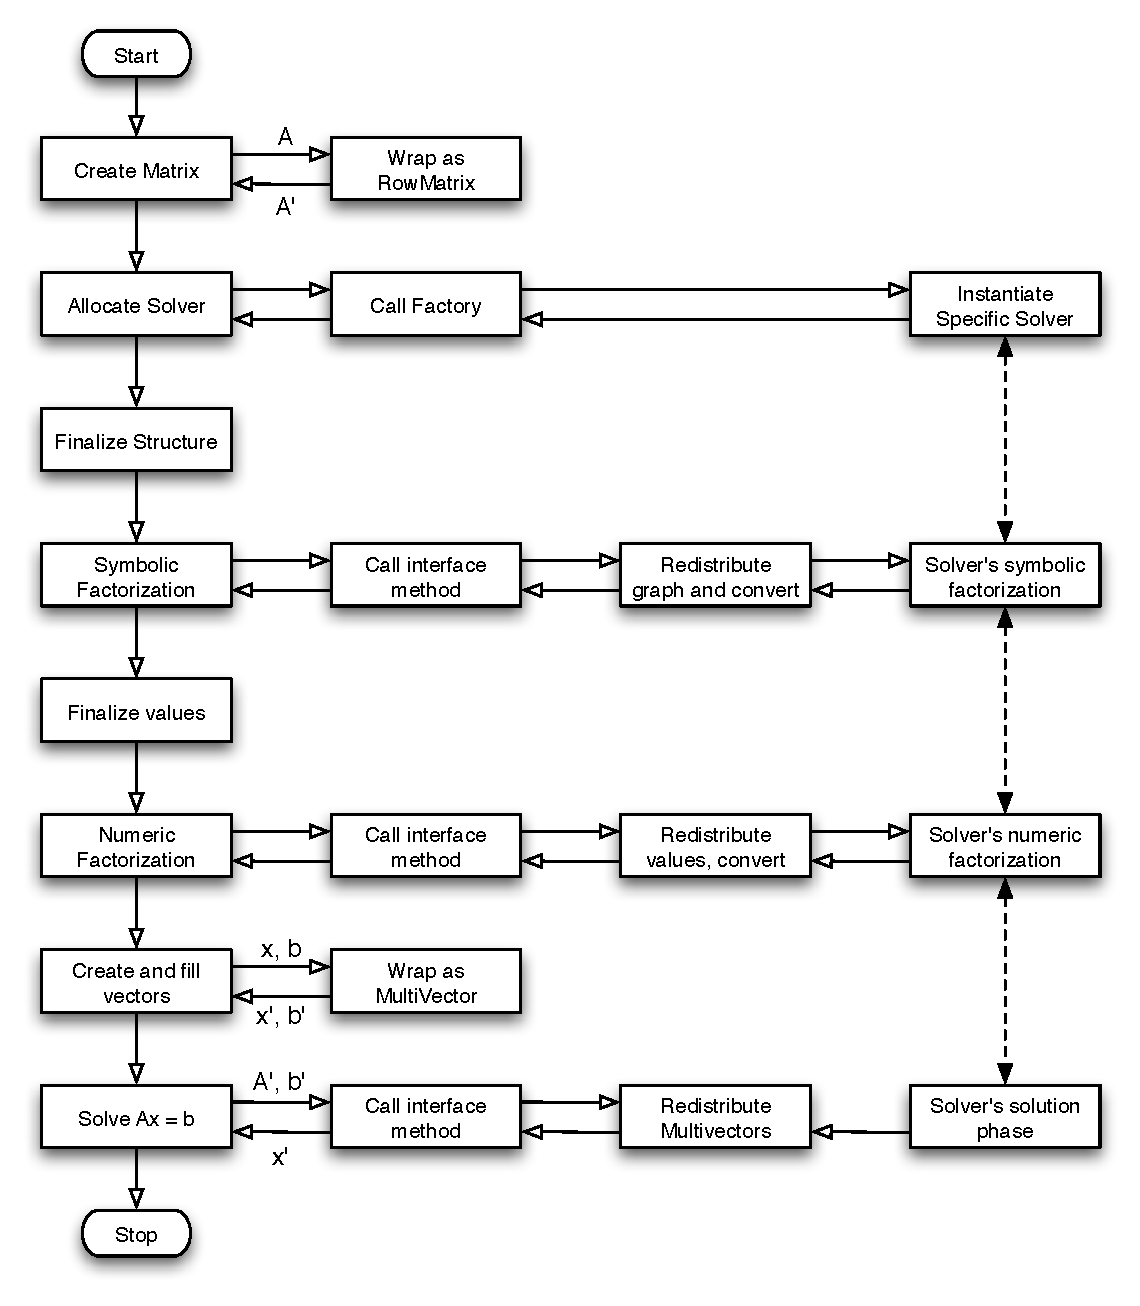
\includegraphics[width=12cm]{amesos_flowchart.pdf}}
\end{center}
\caption{Flowchart of linear system solution. $A, x$ and $b$ represent objects
  defined in the application, while $A', x'$ and $b'$ are the corresponding
    wrappers that
    satisfy Interfaces~\ref{int:vector} and \ref{int:ami}. Dashed lines mean
    that a given phase uses data defined in another phase. From left to right,
  the first column
    represents phases occurring in the application; the second column wrapping
and calls to generic interface methods; the third column actions
occurring in the solver interface, while the fourth column calls to the supported
direct solver library.}
\label{fig:flowchart}
\end{figure}

%-------------------------------------------------------------------------
\section{A Concrete Implementation}
\label{sec:concrete}
%-------------------------------------------------------------------------

We now describe a concrete implementation of the interfaces of
Section~\ref{sec:design}, as implemented in
the {\sl \amesos}\footnote{
\amesos\ is a Greek term that loosely translated means ``direct.''} package~\cite{Amesos-Reference-Guide}.
\amesos,
developed by M.~Heroux, K.~Stanley,
M.~Sala, and R.~Hoekstra, is distributed within the
Trilinos project~\cite{heroux05trilinos} and is available for public
download~\cite{amesos-web-page}.

We have considered the following direct solvers:
  KLU\footnote{KLU source code is
  distributed with \amesos.} \cite{davis05klu},
  UMFPACK~\cite{umfpack-home-page}, SuperLU and
  SuperLU\_DIST~\cite{superlu-manual}
  DSCPACK~\cite{dscpack-manual},
  MUMPS~\cite{mumps-manual},
  TAUCS~\cite{irony04parallel,rotkin04design,rozin04locality},
  and PARDISO~\cite{oskl:04-etna,sg:04-fgcs}. An interface to MA28 is
  under development.
These libraries use different algorithms that are
representative of a far wider range of codes. Also, these supported libraries are
among the best codes publicly available, and are widely used.

\amesos\ also includes interfaces to LAPACK and ScaLAPACK. The rationale is
that
sparse libraries are much more complicated than libraries for dense systems,
  and the question of how much is gained with respect to dense solvers
  is often asked. Dense
  solvers are usually more robust than sparse solvers and could be used as
  last-resort in extreme cases.  By adding support for LAPACK and ScaLAPACK,
  users can experiment with these
  solvers, which might outperform  sparse libraries in some cases
  (for instance, if applied to small matrices, or almost dense matrices).

\begin{figure}
\begin{center}
\begin{tabular}{| p{12cm} | }
\hline
 \\
\begin{minipage}{12cm}
\begin{verbatim}
#include "Amesos.h"
#ifdef HAVE_MPI
#include "mpi.h"
#include "Epetra_MpiComm.h"
#else
#include "Epetra_SerialComm.h"
#endif
#include "Epetra_Vector.h"
#include "Epetra_CrsMatrix.h"

int main(int argc, char *argv[])
{
  MPI_Init(&argc, &argv);
  Epetra_MpiComm comm(MPI_COMM_WORLD);
  int indexBase = 0; // indices start from 0

  // specifies the global size of the problem
  int numGlobalElements n = 5 * Comm.NumProc();
  // creates map, Interface 3.1, then the solution vector x and the
  // right-hand side b (Interface 3.2), and the linear system matrix, Int. 3.3
  Epetra_Map map(numGlobalElements, indexBase, comm);
  Epetra_Vector x(map); x.PutScalar(0.0);
  Epetra_Vector b(map); x.Random(0.0);
  Epetra_CrsMatrix A(Copy, map, 0);
  for (int LocalRow = 0; LocalRow < map.NumMyElements(); ++LocalRow) {
    int GlobalRow = map.GID(LocalRow); // local-to-global mapping
    A.InsertGlobalElements(GlobalRow, 1, 1.0, GlobalRow);
  }
  A.FillComplete();

  Epetra_LinearProblem problem(A, x, b); // Interface 3.4

  Amesos factory;                  // create a factory class
  string solverType = argv[1];     // selected interface, for ex. "Umfpack"
  Amesos_BaseSolver* solver;       // generic solver object, Int. 3.5
  solver = factory.create(solverType, problem); // create solver

  Teuchos::ParameterList list;     // allocate container for params,
  list.set("PrintTiming", true);   // set one in the container, then
  solver->setParameters(list);     // pass the container to the solver

  solver->symbolicFactorization(); // symbolic factorization
  solver->numericFactorization();  // numeric factorization
  solver->solve();                 // linear system solution
  delete solver;

  MPI_Finalize();
  return(EXIT_SUCCESS);
} // end of main()
\end{verbatim}
\end{minipage} \\
 \\
 \hline
\end{tabular}
\caption{Compilable example of code using the \amesos\ interface
  to solve a linear system. The solver is specified run-time as first
argument of the command line. The map contains {\tt
numGlobalElements} elements, in this case distributed linearly. The
right-hand side is a random vector, and the matrix is a simple
diagonal matrix, stored using the {\tt Epetra\_CrsMatrix} format. Note that the {\tt
Epetra} implementation of Interface \ref{int:map} uses {\tt NumMyElements()}
instead of {\tt getNumMyElements()} and {\tt GID()} instead of {\tt getGID()}.}
\label{fig:example}
\end{center}
\end{figure}

To increase portability, \amesos\ is configured using
Autoconf~\cite{Autoconf} and Automake~\cite{Automake}; each
interface can be enabled or disabled at configure time. Users can
take advantage of the bug-tracking tool Bugzilla~\cite{Bugzilla} to
provide feedback or request improvements.

\medskip

\amesos\ provides an abstraction for Interface~\ref{int:asi}, as
well as all its concrete implementations (for a little more than
13,000 code lines, including comments and Doxygen
documentation), and it takes advantage of the {\sc Epetra}
package~\cite{Epetra-Ref-Guide} to implement
Interfaces~\ref{int:map}, \ref{int:vector}, \ref{int:ami} and
\ref{int:lp}. {\sc Epetra} defines several concrete implementations
of Interface~\ref{int:ami}, making it easy to read matrices from
formats
  like AIJ or CSR.
The Standard Template Library (STL)~\cite{wise96overview} is used to
increase performance whenever possible. The \amesos\ implementation
of Interface~\ref{int:asi} also contains methods {\tt PrintStatus()}
and {\tt PrintTiming()} that offer a standard way to access various
statistics and timings for all packages.

An example of usage of \amesos\ is reported in
Figure~\ref{fig:example}. This simple example shows how to define a
distributed linear system. For the sake of simplicity, the linear
system matrix is diagonal; however it is easy to modify the code for
more general cases. Note that a basic usage of \amesos\ only
requires a basic knowledge of the Epetra and Teuchos packages of
Trilinos; see for example~\cite{Trilinos-Tutorial}. The example can
be compiled with or without MPI by properly defining \verb!HAVE_MPI!.
(\amesos\ itself can be compiled with or without support for MPI.
Clearly, distributed solvers are available only when compiled with
MPI support.) When compiled with MPI support and a serial solver
(e.g., UMFPACK) is selected, then \amesos\ will take care of
gathering the distributed linear system to processor 0 and perform
the required actions. Although the example uses the
\verb!Epetra_CrsMatrix! to define the matrix, any class that
satisfies Interface~\ref{int:ami} can indeed be used. It is indeed
quite easy to write wrappers for matrices that have quick access to
row entries. Note that \verb!IndexBase! variable, which defines the
base index. This value is typically set to 0, but it can  be 1 when
FORTRAN arrays are to be used and one seeks to minimize the index
conversion\footnote{{\tt indexBase} refers to the base index for the
global numbering; the local numbering is always set to 0.}.

The only \amesos\ include file is \verb!Amesos.h!, which does not include the
header files of the supported library. The required interface is specified by
the string variable \verb!SolverType!, and is created by using the factory
class \verb!Amesos!. Factory classes are a programming
tool~\cite{alexandrescu01modern} that implements a sort of ``virtual
constructor,'' in the sense that one can instantiate a derived (concrete)
object while still working with abstract data types. The example reported in
Figure~\ref{fig:example} adopts UMFPACK as a solver; however by using the
factory class, other interfaces can be created by simply changing the
parameter {\tt solverType}. Note that the supported solver can be serial or
parallel, dense or sparse: the user code still remains the same, except for
the name of the solver; \amesos\ will take care of data redistribution if
required by the selected solver.

\begin{figure}
\begin{center}
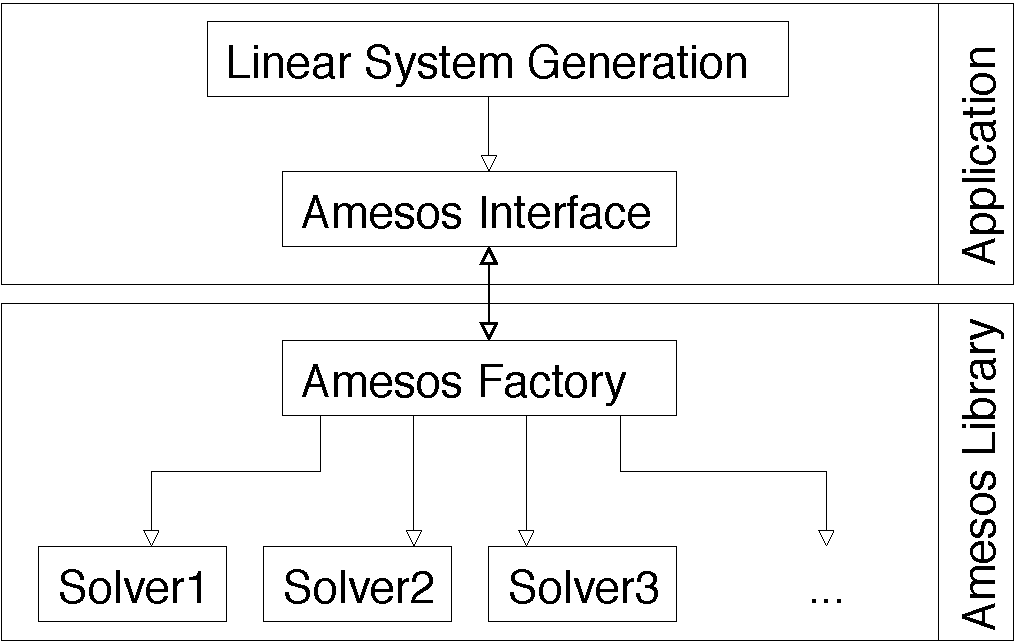
\includegraphics[width=6cm]{amesos_and_application.pdf}
\end{center}
\caption{Connection between a generic application and \amesos.}
\label{fig:app}
\end{figure}

A generic interface between an application code and \amesos\ is as
represented in Figure~\ref{fig:app}: Once $A$, $x$ and $b$ of
(\ref{eq:linear_system}) are available, the application can use the
factory to access any of the supported libraries.

Each \amesos\ interface automatically selects the default parameters
defined by the supported solver. If required, the user can tune some
of the parameters by using the method \verb!setParameters()!. The
list of supported parameters is reported
in~\cite{Amesos-Reference-Guide}.

Using the \verb!setParameters()! we can also set special parameters
that are only recognized by one or a few of the specific solvers.
For example, if we want SuperLU to perform equilibration, we can
pass the required parameter setting to a SuperLU solver through the
generic Amesos solver interface.  Other solvers will not recognize
this parameter if it is passed to them, but this is not a fatal
error.  In this way we can provide custom information to a specific
solver without giving up the generic interface.

One supposed advantage of object-oriented abstract interfaces is
extensibility.  Presently Amesos provides a very high level
interface that is easily supported by any of the solver packages of
interest.  As mentioned above, parameter lists allow us to support
unique capabilities in specific solvers.  However, presently we are
unable to provide much else in terms of custom behavior.  For
example, at this point we are unable to mix-and-match steps from one
concrete solver with another. In other words, we cannot use the
equilibration techniques in SuperLU with UMFPACK. Without greater
commonality in data structures, and agreement on lower level
interfaces across these solver packages, such a goal is difficult to
accomplish.  At the same time, the existence of interface layers
such as Amesos do move us a small step in the direction of interface
standardization that might one day permit this capability.

Extensibility in the form of adding support for another solver is
very straight-forward and our work in this direction continues.
Future versions of Amesos will also support some lower level
computations, in particular multiplication and solve with just the
lower and upper triangles of the factorization.  Such computations
are important for some algorithms and supported by most of the
solver packages available via Amesos.

% ------------------------------------------------------------------------
\section{Numerical Results}
\label{sec:numerical}
% ------------------------------------------------------------------------

The example code of Figure~\ref{fig:example} has shown the facility of usage
of \amesos; this section, instead, aims to quantify its overhead.

Figures~\ref{fig:results1} and \ref{fig:results2} reports the
percentage of CPU time required by the \amesos\ interface with
respect to the time required by the underlying library. We have
considered the SuperLU and UMFPACK interface for the solution of all
matrices in the FIDAP collection, available
at~\cite{boisvert97matrix}. The matrix sizes range from 27 ({\tt
FIDAP005}) to 22294 ({\tt FIDAPM11}), with approximately 20 nonzero
entries per row with just a few exceptions, one of them being at
size 1733 where there are only 10 nonzeros per row and the overhead
cost for SuperLU spikes up to 13\% in Figure~\ref{fig:results1}. All
problems are solved using a 1.67 GHz G4 processor with 1024 Mbytes
of RAM, running MAC OS X 10.4 and gcc 4.0.0. The table reports the
percentage of the CPU time required by the interface with respect to
the time required by the considered solver, and quantifies the
overhead required by \amesos. We have used the default set of
parameters for both solvers.

As expected, for small matrices (for example \verb!FIDAP005! or \verb!FIDAPM05!, of size
27 and 42, respectively)
the overhead is considerable. When considering bigger matrices ($n > 3000$),
then the overhead is  always below 5\%. All the overhead is spent in
converting the matrix from the abstract format of Interface~\ref{int:ami} to the
format required by the library, and performing additional safety checks.
Note that this overhead can indeed be reduced by adding specialized classes,
     that satisfies Interface~\ref{int:ami} but internally store the matrix
     in the format required by a given solver library. Solvers derived from
     Interface~\ref{int:asi} can perform a {\tt dynamic\_cast}, and then get
     the already allocated data structure containing the matrix. This solution
     is inelegant and requires knowledge of derived classes in the solver
     interface, but could greatly increase performance.  Vectors are less
     problematic since Interface \ref{int:vector} already offers the ability
     to get the raw pointers required by the supported library. However, these
     vectors may need to be redistributed to match a given solver's
     requirements.

\begin{figure}
\begin{center}
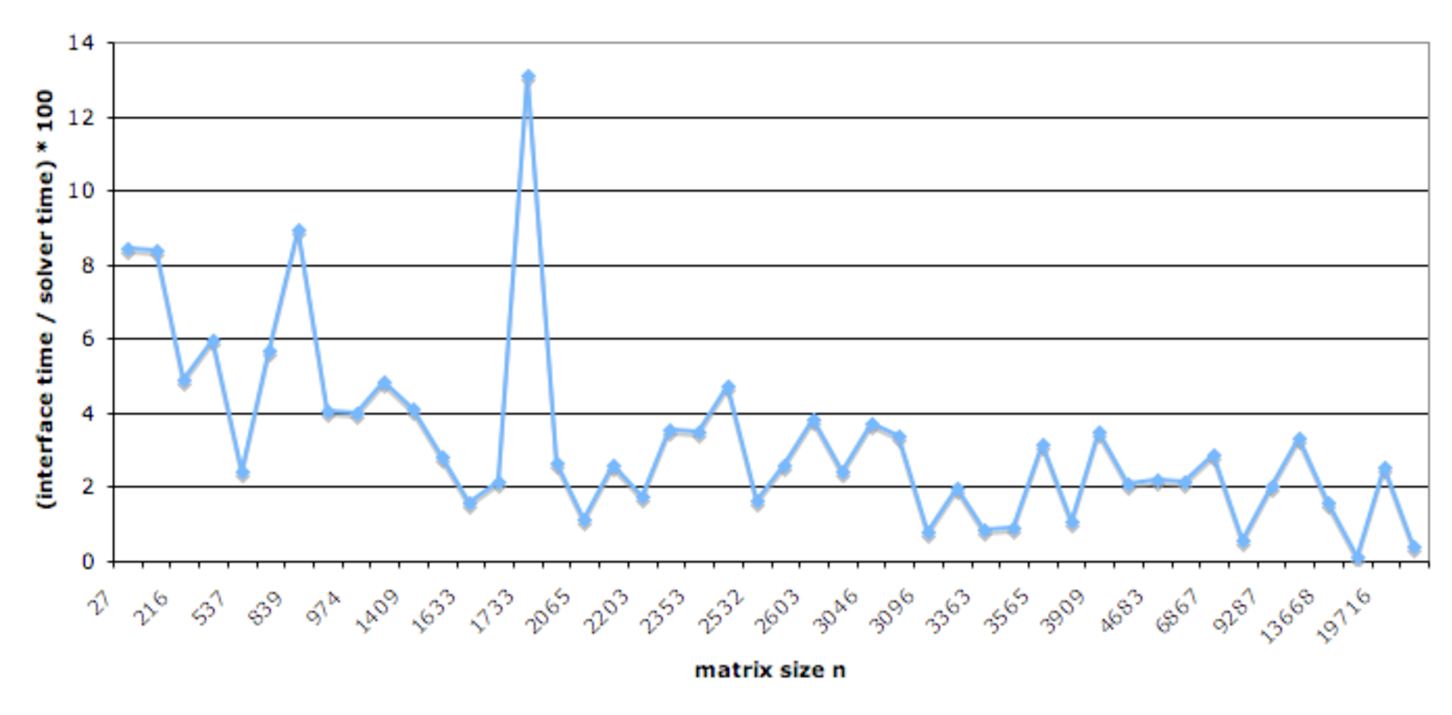
\includegraphics[width=12cm]{superlu_time.pdf}
\caption{Additional time required by the \amesos\ interface with respect to the
time required by the SuperLU solver as a
  function of the matrix size $n$.
The results were obtained on a G4 1.67 GHz with 1 GByte of RAM.}
\label{fig:results1}
\end{center}
\end{figure}

\begin{figure}
\begin{center}
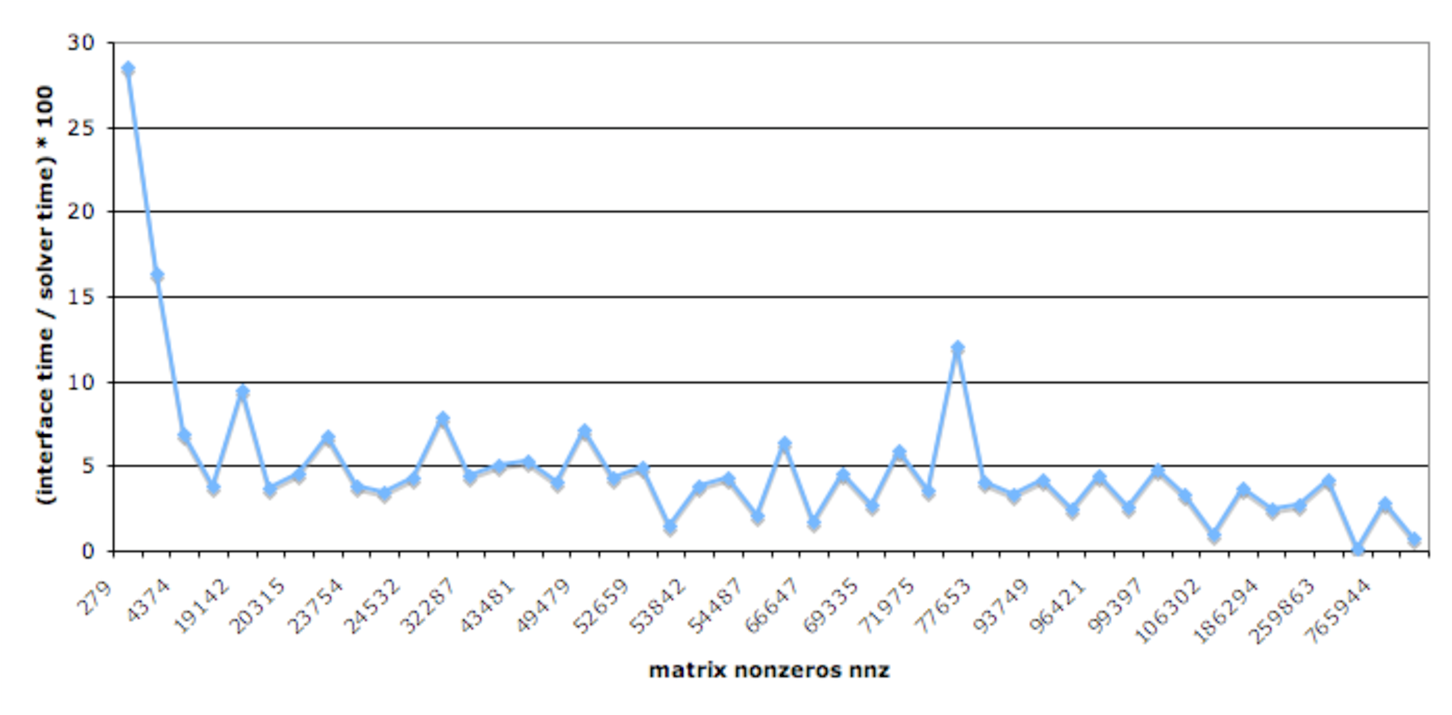
\includegraphics[width=12cm]{umfpack_time.pdf}
\caption{Additional time required by the \amesos\ interface with respect to the
time required by the UMFPACK solver,  as a function of the matrix
  nonzeros $nnz$.
The results were obtained on a G4 1.67 GHz with 1 GByte of RAM.}
\label{fig:results2}
\end{center}
\end{figure}

%-----------------------------------------------------------------------------
\section{Examples of Applications}
\label{sec:example}
%-----------------------------------------------------------------------------

%-----------------------------------------------------------------------------
\subsection{Applications to Domain Decomposition and Multilevel Preconditioners}
\label{sec:preconditioner}
%-----------------------------------------------------------------------------

From an abstract point of view, an algebraic domain decomposition
preconditioner for the iterative solution of the linear system
(\ref{eq:linear_system})
is any preconditioner $B$ that can be written as
\begin{equation}
\label{eq:prec}
B^{-1} = \sum_{i=1}^M P'_i {A'_i}^{-1} R_i,
\end{equation}
where
$M$ is the number of subdomains, $R_i$ is the restriction to subdomain $i$,
  $P_i = R_i^T$, $P_i'$ an auxiliary prolongator operator, and
$A'_i$ an approximation to $A_i = R_i A P_i$.  We refer to
monographs~\cite{QV2,smith96parallel} for a detailed
overview of domain decomposition methods, and to~\cite{saad96iterative} for their
algebraic interpretation.

One disadvantage of one-level domain decomposition preconditioners
is that their performance deteriorates as the number of subdomains
increases. Therefore, these preconditioners are completed by one or
more additional (coarser) levels, as done in two-level domain
decomposition preconditioners or in multilevel methods; see for
instance \cite{brandt.classic,hack.book}.

Direct solution methods can therefore be required in two distinct phases: In the application of
the $A'_i$'s, and in the solution of the coarse problem. In both cases, it
suffices to wrap the $A'_i$'s or the coarse matrix to satisfy
Interface~\ref{int:ami} in order to access to any of the libraries
supported by \amesos. This will be done by using a sequence of instructions that basically looks
like the one shown in Figure~\ref{fig:example}, with the only difference that
the vectors \verb!x! and \verb!b! must be specified just before a call to
\verb!Solve()!.  The libraries IFPACK~\cite{ifpack-guide} and
ML~\cite{ml-guide} are two examples of preconditioning packages adopting this
approach.

%-----------------------------------------------------------------------------
\subsection{Scripting Language Interface: PyAmesos}
\label{sec:pyamesos}
%-----------------------------------------------------------------------------

Another advantage of the presented set of interfaces is the ease with which
they can be used from inside a scripting language like Python by adopting
tools like SWIG~\cite{swig}. This approach makes all the supported libraries
available to Python developers at almost no cost. For more details, we refer
to the PyTrilinos documents~\cite{sala05pytrilinos,pytrilinos-la-guide}.  An
example of usage is reported in Figure~\ref{fig:pyamesos}. The example reads a
matrix in Harwell/Boeing format~\cite{duff89sparse}, distributes it linearly
across the available processors, then calls MUMPS to solve the linear system.
Python's dictionaries are used to specify parameters (in this case, the level
                                                      of output). Note that,
  since SWIG supports intra-language class inheritance, it is possible to
  derive Interfaces~\ref{int:vector} and~\ref{int:ami} in Python, and then pass it to the Python
  wrapper of Interface~\ref{int:asi}.

\begin{figure}
\begin{center}
\begin{tabular}{| p{12cm} |}
\hline
\\
\footnotesize
\begin{minipage}{11.5cm}
\begin{verbatim}
#! /usr/bin/env python
from PyTrilinos import Amesos, Triutils, Epetra

Comm = Epetra.PyComm()
Map, A, x, b, Exact = Triutils.ReadHB("fidap035.rua", Comm)

Problem = Epetra.LinearProblem(A, x, b);
Factory = Amesos.Factory()
SolverType = "MUMPS"
Solver = Factory.Create(SolverType, Problem)
AmesosList = {
  "PrintTiming": True,
  "PrintStatus": True
}
Solver.SetParameters(AmesosList)
Solver.SymbolicFactorization()
Solver.NumericFactorization()
Solver.Solve()
\end{verbatim}
\end{minipage}
\\
\\
\hline
\end{tabular}
\caption{Complete script that solves a linear system using \amesos/MUMPS in
  Python.}
\label{fig:pyamesos}
\end{center}
\end{figure}

%-----------------------------------------------------------------------------
\section{Concluding Remarks}
\label{sec:conclusions}
%-----------------------------------------------------------------------------

In this paper, we have presented a model to access direct solver
libraries. The model is composed of five abstract interfaces. The
advantages of this model are the following:
\begin{itemize}

\item The actual data storage format of the linear system matrix becomes largely unimportant.
Each concrete implementation will take care, if necessary, to convert the
input matrix to the required data format. This means that the
application can choose {\sl any} matrix format that can be wrapped by the
abstract matrix interface.

\item Issues like diagonal perturbations, dropping, reordering or
fill-reducing algorithms can be easily introduced within the
abstract matrix interface. For example, a dropping strategy or a
modification of the diagonals simply requires a new
\verb!getMyRow()! method, without touching the actual matrix
storage. Also, reordering techniques can be implemented and tested
independently of the library used to perform the factorization.

\item The actual calling sequence required by each library to factor the
matrix and solve the linear system is no longer exposed to the user, who only
has to call methods \verb!SymbolicFactorization()!, \verb!NumericFactorization()! and
\verb!Solve()!.

\item Interfaces can be tested more easily because they are all located within
the same library and not spread out into several application codes. The
framework is also quite easy to learn and use, since a basic usage
requires about 20 code lines (see the example of Figure~\ref{fig:example}).

\item It is easy to compare different solvers on a given set of problems. The
\amesos\ distribution contains a (working) template that reads a linear system
from file in the popular Harwell/Boeing format~\cite{duff89sparse} and solves it with all the
enabled solvers. Users can easily modify this template to numerically evaluate
the optimal library for {\sl their} problems.

\item
The framework can serve users with different levels of expertise, from the
usage of libraries as black-box tools, to a fine-tuning of each library's
parameters.

\item
The framework can be easily extended to incorporate libraries for the
resolution of over-determined and under-determined systems. Solving such
systems may involve algorithms other than Gaussian eliminations; nevertheless,
the interfaces will remain almost untouched.

\end{itemize}

The generality of the proposed model comes at a price. The presented model has the following
limitations:
\begin{itemize}
\item
Overhead may be introduced when converting or redistributing the
matrix and/or the vectors into the library's format. For very large
matrices, this can constitute a problem especially in terms of
memory consumption, but is often not a first-order concern.
\item
Fine-tuning of solver's parameters can be
difficult since Interface~\ref{int:asi} has no knowledge of the underlying
solver data structure. Also, we offer no ``intelligent'' way of setting these
parameters.  Projects like the GRID/TLSE~\cite{dayde04overview} can provide
insight on the choice of parameters.

\item There
  is no standard way to
  convert MPI communicators defined in C to MPI communicators defined
  in FORTRAN90/FORTRAN95. On some architectures it is difficult or even
  impossible to perform such a task. Some hacks may be required.

\item
It is almost impossible to support different releases of a given software
library, since new functionalities are often made available behind the same
function names. Besides, often a given function change the required arguments
from one version to the next, making it impossible for the linker to select
the appropriate version of the library.

%
%  This bug has been resolved.   I see no reason to mention it at this point.  Ken
%
% \item
% Not all interfaces can be compiled and linked at the same time. Often
% developers of direct solver libraries take advantage of other, smaller
% libraries, that offer common functionalities. Typically, this happens with
% reordering algorithms. Unfortunately,
% it is not uncommon for different solver libraries to request different
% versions of a given reordering algorithm, all codes using the same function
% names. As a result, not all the interfaces can be compiled and used at the
% same time.
\item
Some libraries offer a one-solve routine without storing any data after the
solution is completed; this option is not  supported
by the presented design, but it could be easily added.

\item
There are no capabilities to obtain the $L$, $D$ and $U$ factors, or the
reorderings $P$ and $Q$. This is because each supported package uses a
different storage format and distribution. Reordering and scaling can be made
library-independent by working on Interfaces~\ref{int:ami} and \ref{int:lp}.

\item
Problematic user-package communications. Because of the high-level view, the
code is safer: it is more difficult to make errors or call the solver with the
wrong set of parameters. \amesos\ classes automatically perform safety checks,
and return an error code when something goes wrong. However, it is often
difficult to abstract the error messages from all supported libraries and
report them in a uniform fashion.  \amesos\ tries to return an error code
related to the error type, and print a few information on screen. However,
users still need to consult the library's manual to decode the error messages.

\item FORTRAN wrappers are not available. Our design is based on a set of C++
classes, which are difficult or impossible to translate to FORTRAN77 or
FORTRAN95. However, custom interfaces can be made available for specific
concrete implementations of the presented interfaces. The status of FORTRAN
wrappers may change
with future implementation of the FORTRAN2003 standard.
\end{itemize}

%The reader might wonder why we have limited our attention to direct methods only, and
%we did not include iterative methods as well in the definition of the abstract
%interfaces. The reason is that, although
%being often more performance in terms of CPU time and memory usage, iterative
%solvers are less robust and mich less black-box than direct methods. Most
%iterative methods are developed for PDE-like problems, and might have poor
%performance if applied to more general matrices. However, libraries based on
%the abstract matrix interface exist.
%
%\smallskip

Despite these issues, we find that the presented set of interfaces
brings its users the well-known benefits of reusable libraries.
Thanks to their generality, these interfaces (and the corresponding
codes) can be used to easily connect intricate applications with
state-of-the-art linear solver libraries, in a simple and
easy-to-maintain way. From the point of view of application
developers, the small amount of required code makes it very
convenient to adopt a project like \amesos. For linear solver
libraries' developers  writing one interface for their own solver
can help to make it applicable and testable to a vast range of
applications.

One of our goals in the design of \amesos\ was to reduce the intellectual
effort required to use direct solver libraries. We feel that this objective
has been achieved, and the performance penalty is very limited in most cases.
In our opinion, the only limitation of \amesos\ is that it supports double
precision only, while most direct solvers allows the solution in single
precision and complex arithmetics.  Our model can support single precision and
complex arithmetics (by using templates, for example), and a templated
version of Interfaces~\ref{int:map}--\ref{int:asi} is under
development.

%-----------------------------------------------------------------------------%
\section*{Acknowledgments}
%-----------------------------------------------------------------------------%

The authors wish to thank R.~Hoekstra, T.~Davis and I. Duff for fruitful
discussions and suggestions about the organization of the \amesos\ project. We
thank Oscar Chinellato for several suggestions that helped to improved this
document, and the anonymous referees for their helpful comments.  Part of the
work has been conducted under the financial support of the Sandia National
Laboratories.

%-----------------------------------------------------------------------------%
\bibliographystyle{acmtrans}
\bibliography{paper}
%-----------------------------------------------------------------------------%

\end{document}

\begin{table}
\begin{center}
\begin{tabular}{|l r r r| r r r|}
\hline
\multicolumn{4}{| c |}{Matrix} &
\multicolumn{3}{ c |}{Interface Time / Solver Time * 100} \\
Name  & $n$   & $nnz$  & $nnz / n$  & KLU     & UMFPACK   & SuperLU \\
\hline
\tt FIDAP001 & 216   &   4374 & 20.25 & 23.5   & 6.89  & 4.89  \\
\tt FIDAP002 & 414   & 26831  & 60.84 & 26.6   & 7.92  & 5.96  \\
\tt FIDAP003 & 1821  & 52659  & 28.91 & 18.5   & 4.94  & 2.64  \\
\tt FIDAP004 & 1601  & 32287  & 20.16 & 1.47   & 4.40  & 2.81  \\
\tt FIDAP005 & 27    & 279    & 10.33 & 112.52 & 28.5  & 8.46  \\
\tt FIDAP006 & 1651  & 49479  & 29.96 & 1.03   & 7.17  & 2.14  \\
\tt FIDAP007 & 1633  & 54487  & 33.36 & 12.8   & 2.07  & 1.59  \\
\tt FIDAP008 & 3096  & 106302 & 34.33 & 10.8   & 0.931 & 0.789 \\
\tt FIDAP009 & 3363  & 99397  & 29.55 & 14.6   & 4.78  & 0.863  \\
\tt FIDAP010 & 2410  & 54816  & 22.74 & 25.78  & 6.43  & 4.75  \\
\tt FIDAP011 & 16614 &1091362 & 65.68 & 0.120  & 0.701 & 0.111 \\
\tt FIDAP012 & 3973  & 80151  & 20.17 & 0.216  & 3.34  & 2.07  \\
\tt FIDAP013 & 2568  & 75628  & 29.45 & 18.31  & 12.1  & 2.59  \\
\tt FIDAP014 & 3251  & 66647  & 20.50 & 0.172  & 1.71  & 1.94  \\
\tt FIDAP015 & 6867  & 96421  & 14.04 & 10.480 & 4.38  & 2.89  \\
\tt FIDAP018 & 5773  & 69335  & 12.01 & 8.18   & 2.73  & 2.14  \\
\tt FIDAP019 & 12005 & 259863 & 21.64 & 15.17  & 4.23  & 3.34  \\
\tt FIDAP020 & 2203  & 69579  & 31.58 & 1.32   & 5.89  & 1.77  \\
\tt FIDAP021 & 656   & 19142  & 29.17 & 6.84   & 9.52  & 5.68  \\
\tt FIDAP022 & 839   & 22613  & 26.95 & 6.50   & 6.76  & 8.92  \\
\tt FIDAP023 & 1409  & 43481  & 30.85 & 0.934  & 5.26  & 4.13  \\
\tt FIDAP024 & 2283  & 48733  & 21.34 & 2.11   & 4.09  & 3.55  \\
\tt FIDAP025 & 848   & 24532  & 28.92 & 9.93   & 4.29  & 4.04  \\
\tt FIDAP026 & 2163  & 93749  & 43.34 & 0.724  & 4.16  & 2.59  \\
\tt FIDAP027 & 974   & 40736  & 41.82 & 5.25   & 5.10  & 4.02  \\
\tt FIDAP028 & 2603  & 77653  & 29.83 & 0.896  & 4.08  & 3.81  \\
\tt FIDAP029 & 2870  & 23754  & 8.276 & 9.95   & 3.81  & 2.44  \\
\tt FIDAP031 & 3909  & 115299 & 29.49 & 0.575  & 3.75  & 3.51  \\
\tt FIDAP032 & 1159  & 11343  & 9.786 & 0.791  & 3.87  & 4.84  \\
\tt FIDAP033 & 1733  & 20315  & 11.72 & 15.89  & 4.58  & 13.1   \\
\tt FIDAP035 & 19716 & 218308 & 11.07 & 8.56   & 2.74  & 2.53  \\
\tt FIDAP036 & 3079  & 53851  & 17.48 & 2.03   & 4.30  & 3.35  \\
\tt FIDAP037 & 3565  & 67591  & 18.95 & 11.08  & 4.58  & 3.15  \\
\tt FIDAPM02 & 537   & 19241  & 35.83 & 14.74  & 3.67  & 2.42  \\
\tt FIDAPM03 & 2532  & 50380  & 19.89 & 1.00   & 4.33  & 1.61  \\
\tt FIDAPM05 & 42    & 520    & 12.38 & 82.85  & 16.3  & 8.40  \\
\tt FIDAPM07 & 2065  & 53533  & 25.92 & 0.602  & 1.52  & 1.15  \\
\tt FIDAPM08 & 3876  & 103076 & 26.59 & 0.220  & 3.36  & 1.08  \\
\tt FIDAPM09 & 4683  & 95053  & 20.29 & 0.536  & 2.45  & 2.21  \\
\tt FIDAPM10 & 3046  & 53842  & 17.67 & 9.979  & 3.82  & 3.72  \\
\tt FIDAPM11 & 22294 & 623554 & 27.96 & N/C    & 0.17  & 0.403 \\
\tt FIDAPM03 & 3549  & 71975  & 20.28 & 0.355  & 3.59  & 0.919 \\
\tt FIDAPM05 & 9287  & 98519  & 10.60 & 42.90  & 2.59  & 2.03  \\
\tt FIDAPM29 & 13668 & 186294 & 13.62 & 0.869  & 2.511 & 1.57  \\
\tt FIDAPM33 & 2353  & 23765  & 10.09 & 0.6560 & 3.39  & 3.47  \\
\tt FIDAPM37 & 9152  & 765944 & 83.69 & 2.247  & 2.87  & 0.585 \\
\hline
\end{tabular}
\end{center}
\end{table}
